\documentclass[12pt]{beamer}
\usepackage{ceai-beamer}
\usepackage{ragged2e}
\AtBeginEnvironment{frame}{\justifying}
\AtBeginSection[]{}
\AtBeginSubsection[]{}

\title[Topic 16: Modern LLM Systems]{CE 488/5588: Applied AI\\Topic 16: Modern LLM Systems and Direct Engineering Applications --- Workflows, Retrieval, and First-Generation AI Engineering}
\author{}
\date{}

\newcommand{\source}[1]{\vspace{0.4em}{\tiny\color{gray}Source: #1\par}}

\begin{document}

\begin{frame}
  \titlepage
\end{frame}

\begin{frame}{Lecture Roadmap}
  \tableofcontents
\end{frame}

\section{From Topic 15 to Topic 16}

\begin{frame}{From Representation to Systems}
  Topic 15 focused on representation:
  \begin{itemize}
    \item how text becomes tokens,
    \item how tokens become vectors,
    \item how vectors support retrieval.
  \end{itemize}

  Topic 16 asks a different question:
  \begin{itemize}
    \item how are modern LLM systems actually organized,
    \item and how do those systems already change engineering work?
  \end{itemize}
\end{frame}

\begin{frame}{Why Topic 16 Matters}
  In practice, an engineering assistant is rarely just a raw pretrained model.

  A usable system usually includes:
  \begin{itemize}
    \item prompting structure,
    \item post-training,
    \item retrieved evidence,
    \item external tools,
    \item human supervision.
  \end{itemize}

  \begin{conceptbox}{Main Shift}
    Topic 16 is about the system stack around the model, not only the model itself.
  \end{conceptbox}
\end{frame}

\begin{frame}{What This Chapter Covers}
  This chapter focuses on direct LLM applications and first-generation LLM engineering.

  It covers:
  \begin{itemize}
    \item mainstream transformer families,
    \item base models versus post-trained assistants,
    \item prompt engineering as workflow design,
    \item ReAct, RAG, and knowledge graphs,
    \item coding and document-centered engineering applications,
    \item the transition toward Topic 17 and more agentic systems.
  \end{itemize}
\end{frame}

\begin{frame}{Why LLM Systems Are More Than Chatbots}
  \begin{figure}
    \centering
    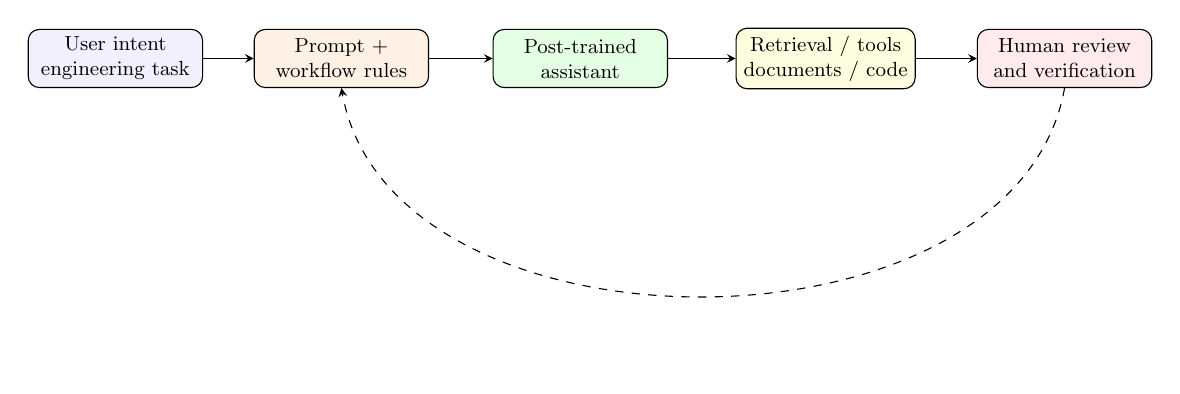
\begin{tikzpicture}[>=stealth,font=\small, scale=0.82, transform shape]
      \tikzset{box/.style={draw, rounded corners, minimum width=2.7cm, minimum height=0.9cm, align=center}}
      \node[box, fill=blue!6] (user) at (0,0) {User intent\\engineering task};
      \node[box, fill=orange!10] (prompt) at (3.5,0) {Prompt +\\workflow rules};
      \node[box, fill=green!10] (assist) at (7.2,0) {Post-trained\\assistant};
      \node[box, fill=yellow!12] (tools) at (11.0,0) {Retrieval / tools\\documents / code};
      \node[box, fill=red!8] (verify) at (14.7,0) {Human review\\and verification};
      \draw[->] (user) -- (prompt);
      \draw[->] (prompt) -- (assist);
      \draw[->] (assist) -- (tools);
      \draw[->] (tools) -- (verify);
      \draw[dashed,->] (verify.south) to[out=-100,in=-80] (prompt.south);
    \end{tikzpicture}
    \caption{A practical system view of an engineering LLM assistant.}
  \end{figure}
\end{frame}

\begin{frame}{Interpreting the System Stack}
  The figure is useful because it makes three practical points explicit:
  \begin{itemize}
    \item prompts organize the interface between the user and the model,
    \item retrieval and tools bring in evidence the model does not reliably store,
    \item verification remains outside the model and inside human responsibility.
  \end{itemize}

  Useful AI engineering begins well before full autonomy.
\end{frame}

\begin{frame}{Learning Objectives}
  After this chapter, students should be able to:
  \begin{itemize}
    \item distinguish encoder-only, decoder-only, and encoder-decoder families,
    \item explain base models versus assistants,
    \item describe prompt engineering as workflow design,
    \item explain RAG and knowledge-graph support for engineering knowledge systems,
    \item describe first-generation engineering workflows such as ReAct,
    \item explain why Topic 17 naturally follows from Topic 16.
  \end{itemize}
\end{frame}

\section{Mainstream Architectures of Modern LLM Systems}

\begin{frame}{Three Main Transformer Families}
  Although people often speak of ``LLMs'' as if they were one architecture, transformer-based systems come in three important families:
  \begin{itemize}
    \item encoder-only,
    \item decoder-only,
    \item encoder-decoder.
  \end{itemize}

  The engineering relevance is that these families are better suited to different task types.

  \source{\href{https://huggingface.co/docs/course/chapter1/6}{Hugging Face Course: Transformer Architectures}}
\end{frame}

\begin{frame}{Encoder-Only Models}
  Encoder-only systems, such as BERT-style models, use bidirectional attention.

  They are strong when the output is mainly an internal representation:
  \begin{itemize}
    \item classification,
    \item semantic similarity,
    \item retrieval,
    \item embedding generation.
  \end{itemize}

  A common objective is masked-token prediction:
  \[
    \mathcal{L}_{\mathrm{MLM}}(\theta) = -\sum_{t\in \mathcal{M}} \log P_\theta(x_t \mid x_{\setminus t}).
  \]
\end{frame}

\begin{frame}{Decoder-Only Models}
  Decoder-only systems, such as GPT-style models, use causal attention.

  This architecture naturally matches autoregressive generation:
  \[
    P(x_1,\dots,x_T) = \prod_{t=1}^{T} P(x_t\mid x_{<t}).
  \]

  This is why decoder-only models became the dominant front end for:
  \begin{itemize}
    \item chat,
    \item coding assistants,
    \item drafting,
    \item general-purpose generation.
  \end{itemize}
\end{frame}

\begin{frame}{Encoder-Decoder Models}
  Encoder-decoder systems, such as T5-style sequence-to-sequence models, split the pipeline into:
  \begin{itemize}
    \item an encoder for the source input,
    \item a decoder for the target sequence,
    \item cross-attention between them.
  \end{itemize}

  Their conditional objective has the form:
  \[
    P(y\mid x) = \prod_{t=1}^{T_y} P(y_t \mid y_{<t}, x).
  \]

  They are especially natural for translation, summarization, and structured text transformation.

  \source{\href{https://huggingface.co/docs/transformers/en/model_doc/encoder-decoder}{Hugging Face: Encoder Decoder Models}}
\end{frame}

\begin{frame}{Architecture Comparison at a Glance}
  \small
  \begin{tabular}{p{0.24\textwidth} p{0.26\textwidth} p{0.34\textwidth}}
    \toprule
    \textbf{Architecture} & \textbf{Main strength} & \textbf{Typical use} \\
    \midrule
    Encoder-only & rich bidirectional representation & embeddings, classification, retrieval \\
    Decoder-only & scalable prompt-driven generation & chat, coding, general assistants \\
    Encoder-decoder & explicit input-to-output mapping & translation, summarization, structured generation \\
    \bottomrule
  \end{tabular}
\end{frame}

\begin{frame}{Three Mainstream Transformer Families}
  \begin{figure}
    \centering
    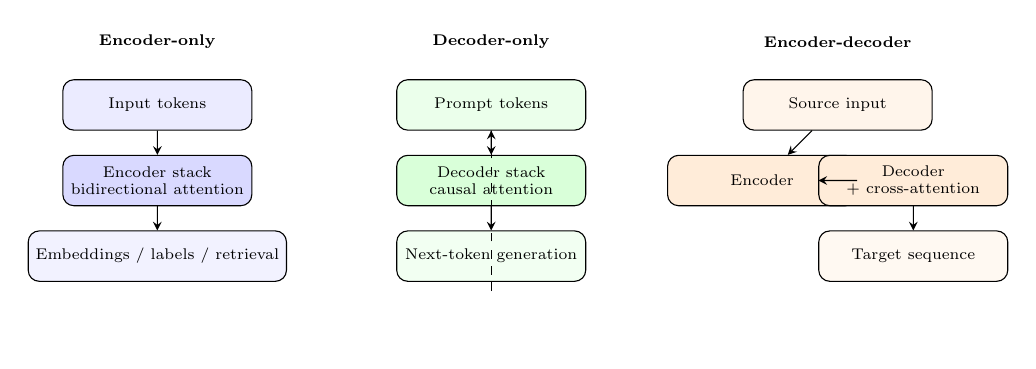
\begin{tikzpicture}[>=stealth,font=\scriptsize, scale=0.80, transform shape]
      \tikzset{box/.style={draw, rounded corners, minimum width=3.0cm, minimum height=0.8cm, align=center}}
      \node[box, fill=blue!8] (encin) at (0,2.0) {Input tokens};
      \node[box, fill=blue!15] (enc) at (0,0.8) {Encoder stack\\bidirectional attention};
      \node[box, fill=blue!5] (encout) at (0,-0.4) {Embeddings / labels / retrieval};
      \draw[->] (encin) -- (enc);
      \draw[->] (enc) -- (encout);
      \node at (0,3.0) {\textbf{Encoder-only}};

      \node[box, fill=green!8] (decin) at (5.3,2.0) {Prompt tokens};
      \node[box, fill=green!15] (dec) at (5.3,0.8) {Decoder stack\\causal attention};
      \node[box, fill=green!5] (decout) at (5.3,-0.4) {Next-token generation};
      \draw[->] (decin) -- (dec);
      \draw[->] (dec) -- (decout);
      \draw[dashed,->] (decout.south) to[out=-90,in=-90] (decin.south);
      \node at (5.3,3.0) {\textbf{Decoder-only}};

      \node[box, fill=orange!8] (seqin) at (10.8,2.0) {Source input};
      \node[box, fill=orange!15] (seqenc) at (9.6,0.8) {Encoder};
      \node[box, fill=orange!15] (seqdec) at (12.0,0.8) {Decoder\\+ cross-attention};
      \node[box, fill=orange!5] (seqout) at (12.0,-0.4) {Target sequence};
      \draw[->] (seqin) -- (seqenc);
      \draw[->] (seqenc) -- (seqdec);
      \draw[->] (seqdec) -- (seqout);
      \node at (10.8,3.0) {\textbf{Encoder-decoder}};
    \end{tikzpicture}
    \caption{Three mainstream transformer families.}
  \end{figure}
\end{frame}

\begin{frame}{Why This Architecture Figure Matters}
  The figure is more useful here than a generic transformer diagram because Topic 16 is about system choices.

  \begin{conceptbox}{Design Consequence}
    Different architectural families support different engineering tasks for structural reasons, not just branding reasons.
  \end{conceptbox}

  If the task is embedding and search, encoder-style models are natural. If the task is interactive generation, decoder-only models dominate. If the task is explicit transformation from one text form to another, encoder-decoder models are conceptually clean.
\end{frame}

\begin{frame}{Why Decoder-Only Models Dominated the Public Interface}
  After 2020, decoder-only systems drove the public AI wave because one architecture could support:
  \begin{itemize}
    \item chat,
    \item code completion,
    \item summarization,
    \item drafting,
    \item transformation,
    \item question answering.
  \end{itemize}

  This does not make the other families obsolete. It means decoder-only models became the most versatile public front end.
\end{frame}

\section{Base Models, Post-Training, and Assistant Behavior}

\begin{frame}{Base Model versus Assistant}
  A \textbf{base model} is the raw language model after pretraining.

  A \textbf{post-trained assistant} is what results after additional behavioral shaping:
  \begin{itemize}
    \item instruction following,
    \item formatting reliability,
    \item tone and style preferences,
    \item refusal or safety behavior.
  \end{itemize}

  \begin{conceptbox}{Practical Difference}
    What users experience is not just the architecture. It is the architecture plus post-training.
  \end{conceptbox}
\end{frame}

\begin{frame}{Instruction Tuning}
  Instruction tuning uses prompt-response demonstrations to teach task-following behavior.

  If the training set is $\mathcal{D}$, the supervised objective is:
  \[
    \mathcal{L}_{\mathrm{SFT}}(\theta) = -\sum_{(x,y)\in \mathcal{D}} \log P_\theta(y\mid x).
  \]

  This is the step that helps convert ``a model that can continue text'' into ``a model that behaves like an assistant.''
\end{frame}

\begin{frame}{Preference Optimization}
  Not every desired behavior is a single correct answer.

  Many goals are preference-like:
  \begin{itemize}
    \item helpfulness,
    \item professionalism,
    \item clarity,
    \item concision,
    \item tone.
  \end{itemize}

  RLHF and DPO are both attempts to shape outputs toward what people prefer, not only toward what is statistically likely.
\end{frame}

\begin{frame}{Parameter-Efficient Customization}
  Organizations often want narrow customization without retraining every parameter.

  That is why methods such as LoRA matter in practice:
  \begin{itemize}
    \item lower memory cost,
    \item lower engineering friction,
    \item easier adaptation to domain language,
    \item useful for internal styles, templates, or terminology.
  \end{itemize}
\end{frame}

\begin{frame}{Why This Matters for Engineers}
  For engineering organizations, many real use cases are narrow:
  \begin{itemize}
    \item report templates,
    \item compliance phrasing,
    \item project-specific terminology,
    \item domain-focused code support.
  \end{itemize}

  Those use cases often do not require frontier-scale retraining. They require system design around an already capable model.
\end{frame}

\section{Prompt Engineering as Workflow Design}

\begin{frame}{Prompt Engineering Is Not Magic}
  Prompt engineering is sometimes presented as the search for one magical sentence.

  That is not the most useful engineering view.

  \begin{conceptbox}{Better View}
    Prompt engineering is the design of a workflow interface between human intent and model behavior.
  \end{conceptbox}
\end{frame}

\begin{frame}{Prompt Components}
  A reliable prompt often specifies:
  \begin{itemize}
    \item role,
    \item context,
    \item task,
    \item constraints,
    \item verification cues.
  \end{itemize}

  The point is not mysticism. The prompt acts like a lightweight program written in natural language.

  \source{\href{https://python.langchain.com/docs/concepts/prompt_templates}{LangChain Docs: Prompt Templates}}
\end{frame}

\begin{frame}{A Minimal Prompt Template}
  \small
  \begin{examplebox}{Example Template}
Role: You are a structural engineering assistant.\\
Context: Use only the attached design note and cited code clauses.\\
Task: Summarize the controlling assumptions for serviceability checks.\\
Constraints: Return 5 bullet points and cite the source section for each.\\
Verification: If a needed source is missing, say so explicitly.
  \end{examplebox}

  This is already a workflow: it tells the model what to do, what evidence to use, and how to signal uncertainty.
\end{frame}

\begin{frame}{Structured Prompting Patterns}
  Useful prompting patterns include:
  \begin{itemize}
    \item few-shot prompting,
    \item decomposition prompting,
    \item format-constrained prompting,
    \item verification prompting,
    \item tool-oriented prompting.
  \end{itemize}

  These matter because engineering tasks often require bounded outputs, traceable assumptions, and explicit uncertainty handling.
\end{frame}

\begin{frame}{Prompt Engineering as Workflow Design}
  \begin{figure}
    \centering
    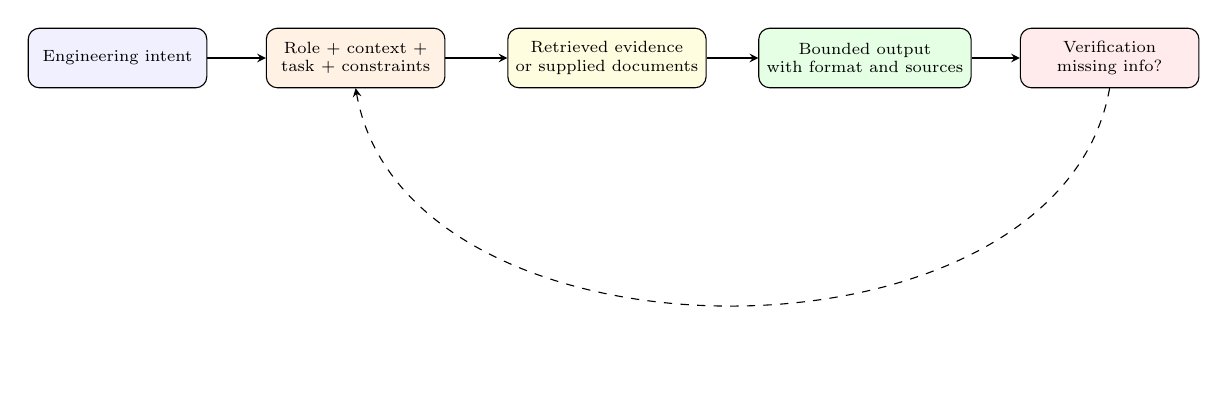
\begin{tikzpicture}[>=stealth,font=\scriptsize, scale=0.84, transform shape]
      \tikzset{box/.style={draw, rounded corners, minimum width=2.7cm, minimum height=0.9cm, align=center}}
      \node[box, fill=blue!6] (intent) at (0,0) {Engineering intent};
      \node[box, fill=orange!10] (schema) at (3.6,0) {Role + context +\\task + constraints};
      \node[box, fill=yellow!12] (evidence) at (7.4,0) {Retrieved evidence\\or supplied documents};
      \node[box, fill=green!10] (output) at (11.3,0) {Bounded output\\with format and sources};
      \node[box, fill=red!8] (check) at (15.0,0) {Verification\\missing info?};
      \draw[->] (intent) -- (schema);
      \draw[->] (schema) -- (evidence);
      \draw[->] (evidence) -- (output);
      \draw[->] (output) -- (check);
      \draw[dashed,->] (check.south) to[out=-100,in=-80] (schema.south);
    \end{tikzpicture}
    \caption{Prompt engineering as workflow design.}
  \end{figure}
\end{frame}

\begin{frame}{Why the Prompt-Workflow Figure Matters}
  The figure emphasizes that a strong prompt does more than ask for an answer.

  It helps organize:
  \begin{itemize}
    \item what evidence matters,
    \item what format is required,
    \item how uncertainty should be expressed,
    \item what counts as success or failure.
  \end{itemize}

  \begin{warningbox}{Important Caution}
    A strong prompt can improve behavior, but it cannot create reliable evidence that is not present in the context.
  \end{warningbox}
\end{frame}

\section{First-Generation LLM Engineering Workflows}

\begin{frame}{Before Full Agents}
  Before frontier autonomous agents became a mainstream topic, many practical LLM workflows already existed.

  These are best understood as \emph{first-generation AI engineering patterns}:
  \begin{itemize}
    \item more structured than ordinary chat,
    \item more tool-aware than plain prompting,
    \item but still short of full autonomy.
  \end{itemize}
\end{frame}

\begin{frame}{ReAct as a Bridge Pattern}
  ReAct stands for \emph{reasoning and acting}.

  The central idea is to interleave reasoning with action:
  \[
    \text{Thought} \rightarrow \text{Action} \rightarrow \text{Observation} \rightarrow \text{Thought} \rightarrow \cdots
  \]

  This makes the workflow iterative, tool-aware, and partially self-correcting.

  \source{\href{https://arxiv.org/abs/2210.03629}{Yao et al. (2023): ReAct}}
\end{frame}

\begin{frame}{A Simplified ReAct Loop}
  \begin{figure}
    \centering
    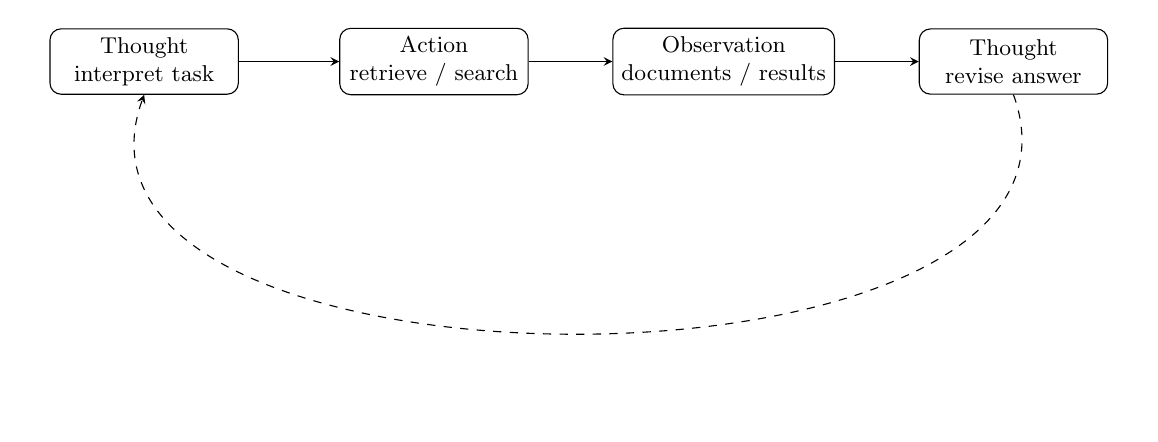
\begin{tikzpicture}[>=stealth,font=\small, scale=0.92, transform shape]
      \tikzset{box/.style={draw, rounded corners, minimum width=2.6cm, minimum height=0.9cm, align=center}}
      \node[box] (t1) at (0,0) {Thought\\interpret task};
      \node[box] (a1) at (4,0) {Action\\retrieve / search};
      \node[box] (o1) at (8,0) {Observation\\documents / results};
      \node[box] (t2) at (12,0) {Thought\\revise answer};
      \draw[->] (t1) -- (a1);
      \draw[->] (a1) -- (o1);
      \draw[->] (o1) -- (t2);
      \draw[dashed,->] (t2.south) to[out=-70,in=-110] (t1.south);
    \end{tikzpicture}
    \caption{A simplified ReAct-style loop.}
  \end{figure}
\end{frame}

\begin{frame}{Why ReAct Matters in Engineering}
  Engineering tasks rarely succeed from one fluent answer.

  The useful workflow is often:
  \begin{itemize}
    \item identify the missing source,
    \item retrieve the clause or document,
    \item inspect the evidence,
    \item revise the answer,
    \item document assumptions.
  \end{itemize}

  ReAct matters because it teaches the system to work with intermediate evidence instead of jumping directly to a final answer.
\end{frame}

\begin{frame}{Engineering Example: Code Compliance}
  \begin{examplebox}{Serviceability Question}
    Suppose a user asks: ``What serviceability deflection limit applies here?''
  \end{examplebox}

  A ReAct-style workflow might:
  \begin{itemize}
    \item retrieve the relevant code section,
    \item observe that the clause depends on occupancy or finish sensitivity,
    \item request or infer that missing context,
    \item produce a bounded answer tied to evidence.
  \end{itemize}
\end{frame}

\section{RAG and Knowledge Bases}

\begin{frame}{RAG as a System Pattern}
  Retrieval-augmented generation combines two ideas:
  \begin{enumerate}
    \item retrieve relevant external documents,
    \item condition generation on those retrieved documents.
  \end{enumerate}

  This shifts the core question from:
  \begin{itemize}
    \item ``What does the model remember?''
    \item to ``What evidence can the system retrieve and use?''
  \end{itemize}

  \source{\href{https://arxiv.org/abs/2005.11401}{Lewis et al. (2020): Retrieval-Augmented Generation}}
\end{frame}

\begin{frame}{A Practical RAG Pipeline}
  \begin{figure}
    \centering
    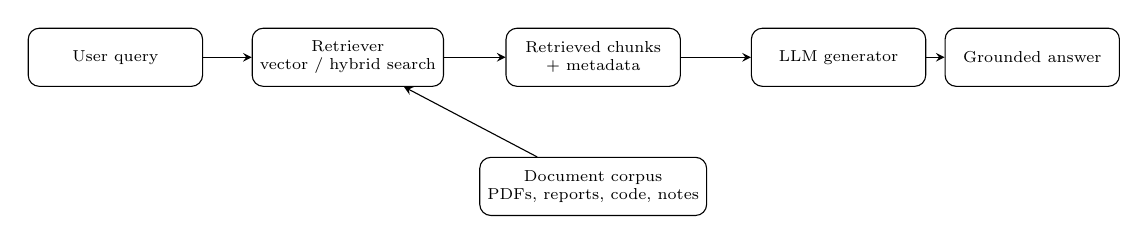
\begin{tikzpicture}[>=stealth,font=\scriptsize, scale=0.82, transform shape]
      \tikzset{box/.style={draw, rounded corners, minimum width=2.7cm, minimum height=0.9cm, align=center}}
      \node[box] (q) at (0,0) {User query};
      \node[box] (r) at (3.6,0) {Retriever\\vector / hybrid search};
      \node[box] (d) at (7.4,0) {Retrieved chunks\\+ metadata};
      \node[box] (g) at (11.2,0) {LLM generator};
      \node[box] (a) at (14.2,0) {Grounded answer};
      \draw[->] (q) -- (r);
      \draw[->] (r) -- (d);
      \draw[->] (d) -- (g);
      \draw[->] (g) -- (a);
      \node[box] (c) at (7.4,-2.0) {Document corpus\\PDFs, reports, code, notes};
      \draw[->] (c) -- (r);
    \end{tikzpicture}
    \caption{A practical RAG pipeline for engineering knowledge work.}
  \end{figure}
\end{frame}

\begin{frame}{Why the RAG Figure Matters}
  The figure highlights a crucial design principle:
  \begin{itemize}
    \item the retriever brings in evidence before generation,
    \item the answer depends on accessible context, not only model memory,
    \item metadata remains part of the practical retrieval story.
  \end{itemize}

  This is why RAG is especially natural for standards, reports, project archives, and office knowledge systems.
\end{frame}

\begin{frame}{LangChain-Style Orchestration}
  Frameworks such as LangChain became popular because they made it easier to connect:
  \begin{itemize}
    \item prompt templates,
    \item retrievers,
    \item tools,
    \item memory,
    \item output formatting.
  \end{itemize}

  The important lesson is not one API. It is the application-layer orchestration pattern.

  \source{\href{https://python.langchain.com/docs/use_cases/more/agents/autonomous_agents/meta_prompt}{LangChain Docs: Build a RAG Agent}}
\end{frame}

\begin{frame}{Engineering Knowledge Bases}
  A useful engineering knowledge base is not just a pile of text.

  It is:
  \begin{itemize}
    \item indexed,
    \item chunked,
    \item traceable,
    \item version-aware,
    \item filtered by source type and authority.
  \end{itemize}

  The technical challenge is not only retrieval quality. It is also governance.
\end{frame}

\begin{frame}{What Governance Means Here}
  For engineering work, a good knowledge system must help distinguish:
  \begin{itemize}
    \item official design codes,
    \item internal office standards,
    \item project-specific memos,
    \item advisory notes,
    \item superseded versus current sources.
  \end{itemize}

  Retrieval quality without source governance is not enough.
\end{frame}

\section{Knowledge Graph Creation with LLMs}

\begin{frame}{Why Knowledge Graphs Matter}
  RAG is not the only way to organize knowledge.

  Knowledge graphs store entities and relations explicitly, often as triples:
  \[
    (h,r,t)
  \]

  Examples:
  \[
    (\texttt{ACI318},\ \texttt{defines},\ \texttt{load\ combination})
  \]
  \[
    (\texttt{Beam\ B12},\ \texttt{uses\ material},\ \texttt{A992\ steel})
  \]
\end{frame}

\begin{frame}{Text to Knowledge Graph Workflow}
  \begin{figure}
    \centering
    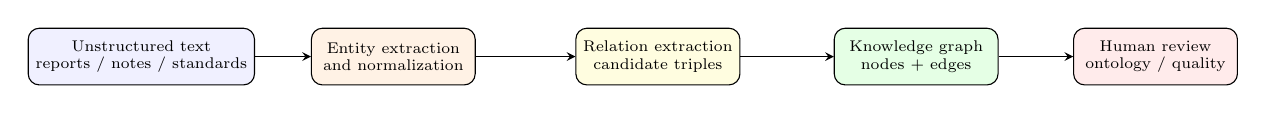
\begin{tikzpicture}[>=stealth,font=\scriptsize, scale=0.80, transform shape]
      \tikzset{box/.style={draw, rounded corners, minimum width=2.6cm, minimum height=0.9cm, align=center}}
      \node[box, fill=blue!6] (text) at (0,0) {Unstructured text\\reports / notes / standards};
      \node[box, fill=orange!10] (entity) at (4.0,0) {Entity extraction\\and normalization};
      \node[box, fill=yellow!12] (relation) at (8.2,0) {Relation extraction\\candidate triples};
      \node[box, fill=green!10] (graph) at (12.3,0) {Knowledge graph\\nodes + edges};
      \node[box, fill=red!8] (review) at (16.1,0) {Human review\\ontology / quality};
      \draw[->] (text) -- (entity);
      \draw[->] (entity) -- (relation);
      \draw[->] (relation) -- (graph);
      \draw[->] (graph) -- (review);
    \end{tikzpicture}
    \caption{A simplified text-to-knowledge-graph workflow.}
  \end{figure}
\end{frame}

\begin{frame}{How LLMs Help Build Graphs}
  LLMs can assist with:
  \begin{itemize}
    \item entity extraction,
    \item relation extraction,
    \item alias resolution,
    \item ontology normalization,
    \item draft triple generation.
  \end{itemize}

  \begin{warningbox}{Important Limitation}
    A graph triple can look formally clean while still being semantically wrong. Human review remains necessary.
  \end{warningbox}
\end{frame}

\begin{frame}{RAG and Knowledge Graphs Are Complementary}
  RAG is strong when you want grounded access to source passages.

  Knowledge graphs are strong when you want:
  \begin{itemize}
    \item explicit relationships,
    \item structured queries,
    \item schema-aware reasoning,
    \item integration with rule-based logic.
  \end{itemize}

  Many useful engineering systems may combine both.
\end{frame}

\section{Direct LLM Applications in Engineering Work}

\begin{frame}{Document-Centered Applications}
  Before autonomy becomes the story, many direct applications already matter:
  \begin{itemize}
    \item summarizing long reports or standards,
    \item extracting assumptions, risks, and action items,
    \item comparing specification revisions,
    \item generating draft technical narratives,
    \item question answering over project archives.
  \end{itemize}

  These applications often create value by reducing knowledge bottlenecks rather than replacing final engineering authority.
\end{frame}

\begin{frame}{Coding and Programming Assistance}
  LLMs are also becoming practical front ends for programming.

  Coding assistants can:
  \begin{itemize}
    \item explain unfamiliar codebases,
    \item draft scripts for analysis or visualization,
    \item translate intent into regex, SQL, or Python,
    \item propose tests, refactors, or documentation,
    \item help navigate multi-file repositories faster.
  \end{itemize}
\end{frame}

\begin{frame}{A Direct Coding-Assistant Workflow}
  \begin{figure}
    \centering
    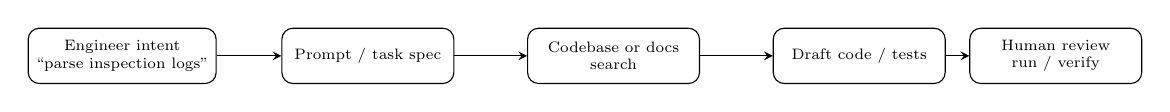
\begin{tikzpicture}[>=stealth,font=\scriptsize, scale=0.78, transform shape]
      \tikzset{box/.style={draw, rounded corners, minimum width=2.8cm, minimum height=0.9cm, align=center}}
      \node[box] (intent) at (0,0) {Engineer intent\\``parse inspection logs''};
      \node[box] (prompt) at (4,0) {Prompt / task spec};
      \node[box] (search) at (8,0) {Codebase or docs\\search};
      \node[box] (draft) at (12,0) {Draft code / tests};
      \node[box] (review) at (15.2,0) {Human review\\run / verify};
      \draw[->] (intent) -- (prompt);
      \draw[->] (prompt) -- (search);
      \draw[->] (search) -- (draft);
      \draw[->] (draft) -- (review);
    \end{tikzpicture}
    \caption{A direct coding-assistant workflow.}
  \end{figure}
\end{frame}

\begin{frame}{Why the Coding Workflow Figure Matters}
  The key point is that this is still a human-directed pipeline.

  Natural-language intent is translated into:
  \begin{itemize}
    \item search,
    \item draft generation,
    \item explicit verification.
  \end{itemize}

  It is more than autocomplete, but it is not yet unconstrained autonomy.
\end{frame}

\begin{frame}{Examples of AI-Native Coding Front Ends}
  Tools such as GitHub Copilot, Claude Code, and OpenCode represent a broader interface shift.

  The user increasingly describes an objective in language, and the system translates that into:
  \begin{itemize}
    \item repository search,
    \item code generation,
    \item edits,
    \item verification steps,
    \item planning support.
  \end{itemize}
\end{frame}

\begin{frame}{Engineering Example: Analysis Assistance}
  \begin{examplebox}{Sensor Drift Study}
    A student wants to compare sensor drift before and after recalibration.
  \end{examplebox}

  Instead of starting from scratch, the assistant can:
  \begin{itemize}
    \item inspect the CSV schema,
    \item write a cleaning function,
    \item generate a plotting routine,
    \item explain assumptions in the analysis.
  \end{itemize}

  The useful output is not only code. It is faster movement from problem description to a runnable workflow.
\end{frame}

\section{Language as Programming, Language as Software}

\begin{frame}{A Broader Conceptual Shift}
  In classical software engineering, programming usually means writing formal code in languages such as Python, C++, or MATLAB.

  In modern LLM workflows, natural language increasingly acts as a specification layer.

  This does not replace formal code. It changes how objectives, constraints, and orchestration are expressed.
\end{frame}

\begin{frame}{Working Thesis}
  \begin{conceptbox}{Language as Software Interface}
    Formal code still executes the work, but natural language increasingly specifies objectives, constraints, orchestration, and interaction patterns.
  \end{conceptbox}

  This matters in engineering because engineering work is already mediated by language: requirements, standards, reports, contracts, and code comments are all part of the computational ecosystem.
\end{frame}

\begin{frame}{Why Topic 17 Must Go Further}
  Topic 16 leaves us with a natural next question:
  \begin{itemize}
    \item if prompts can orchestrate steps,
    \item if retrieval can ground answers,
    \item if ReAct can interleave thought and action,
    \item and if coding assistants can navigate tools,
  \end{itemize}

  what changes when those pieces become persistent, tool-using, and increasingly agentic?
\end{frame}

\begin{frame}{Transition to Topic 17}
  \begin{warningbox}{What Comes Next}
    Topic 16 showed that useful AI engineering begins well before full autonomy. Topic 17 asks what changes when these first-generation workflows become persistent, tool-using, multi-step systems that look increasingly agentic.
  \end{warningbox}

  That is where human-in-the-loop engineering becomes fully concrete.
\end{frame}

\begin{frame}{Chapter Takeaways}
  \begin{itemize}
    \item modern LLM systems are best understood as workflows, not just models,
    \item different transformer families support different task types,
    \item assistants feel different from base models because of post-training,
    \item prompt engineering is workflow design,
    \item ReAct, RAG, and knowledge graphs are first-generation engineering patterns,
    \item direct value often comes from document and coding workflows before autonomy.
  \end{itemize}
\end{frame}

\end{document}
